\chapter{Set Theory and Metric Space}

Set theory and metric space are introduced in this chapter as the preliminaries to general topology. They are also the building blocks of many other mathematics subjects such as algebra and geometry.

\section{Set}

TBA

\section{Metric Space}

Metric space is introduced in this section.

\subsection{Definition}

A \mync{metric space} is a non-empty set $X$ with a distance function $d: X \times X \to \mathbb{R}_{\geq 0}$, where function $d$ satisfies the following properties.
\begin{itemize}
	\item Symmetric: $\forall x, y \in X$, $d(x,y)=d(y,x)$;
	\item Positive definite: $\forall x, y \in X$, $d(x,y)\geq 0$, and $d(x,y)=0$ if and only if $x=y$;
	\item Triangle inequality: $\forall x, y, z \in X$, $d(x,z)\geq d(x,y) + d(y, z)$.
\end{itemize}

\begin{mdframed}
\noindent \textbf{Is metric space an algebraic system?}

No, we do not consider metric space as an algebraic system. 

The distance function defined in a metric space is essentially a mapping but not an operator. The tools and properties we study on metric spaces and algebraic systems are also different.

In that perspective, though both metric space and algebraic system define set and ``rules'' of some kind, they are different.

\end{mdframed}

Consider the following metric space $(X,d)$, where the distance function is defined by
\begin{eqnarray}
	d(x,y) &=& \left\{\begin{array}{cc}
		0 & x=y \\
		1 & \textup{otherwise}
	\end{array}\right.
\end{eqnarray}
It can be easily proved that the above meets the criteria of metric space, hence $(X,d)$ a metric space. This is probably one of the simplest metric spaces and it demonstrates that metric space can be defined on any non-empty set. But of course, this metric space is not very interesting, nor useful.

In the next Sections \ref{sec:p-norm}, \ref{sec:open-set} and \ref{sec:continuous-function}, some important metric spaces defined on vector space are introduced, together with some important definitions introduced as extensions of these metric spaces.

\begin{mdframed}
\noindent \textbf{What is vector space?}

The definition of vector space is introduced first in linear algebra. A recap is given below. A \mync{vector space} refers to an algebraic system with a set of objects called vectors and with the following operators
\begin{eqnarray}
	\oplus &:& V \times V \to V \nonumber \\
	\odot &:& \mathbb{R} \times V \to V \nonumber
\end{eqnarray}
where $\oplus$ is the addition operator that combines two vectors to make a third vector inside the set, and $\odot$ the scalar multiplication operator that scale the vector by a scalar to get a new vector inside the set. Notice that a vector space is always closed under both addition and scalar multiplication.

\end{mdframed}

\subsection{$p$-Norm and $l^p$ Space} \label{sec:p-norm}

\mync{Euclidean distance} (also known as \mync{$l^2$-distance}) is a metric space defined on $\mathbb{R}^n$, with the distance function defined by
\begin{eqnarray}
	\norm{x-y}_2 &=& \left(\sum_n|x_i-y_i|^2\right)^{\frac{1}{2}} \label{eq:euclidean-distance}
\end{eqnarray}
Euclidean distance is one of the most popular metric spaces in science and engineering, and it will be frequently used in the remainder of this notebook, 

Another example of metric space is the \mync{$l^\infty$-distance} on $\mathbb{R}^n$ with the distance function defined by
\begin{eqnarray}
	\norm{x-y}_\infty &=& \max_{n}~|x_i - y_i| \label{eq:l-infinity-distance}
\end{eqnarray}

It can be easily verified that both Euclidean distance and $l^\infty$-distance on $\mathbb{R}^n$ satisfy the definition of metric space.

Both Euclidean distance and $l^\infty$-distance can be derived from \mync{$p$-norm} which is defined on $\mathbb{R}^n$ as follows.
\begin{eqnarray}
	\norm{x}_p &=& \left(\sum_n |x_i|^p\right)^{\frac{1}{p}} \label{eq:p-norm}
\end{eqnarray}
where $p>0$. Under the scope of this notebook, only positive integer $p$ is considered.

Letting $p=2$ in \eqref{eq:p-norm} gives
\begin{eqnarray}
	\norm{x}_2 &=& \left(\sum_n x_i^2\right)^{\frac{1}{2}} \nonumber
\end{eqnarray}
which is known as the \mync{Euclidean norm}, and Euclidean distance in \eqref{eq:euclidean-distance} is the Euclidean norm of $x-y$.

Letting $p\rightarrow \infty$ in \eqref{eq:p-norm} gives
\begin{eqnarray}
	\norm{x}_{\infty} &=& \max_n ~ |x_i| \nonumber
\end{eqnarray}
which is known as the \mync{infinity norm}, and $l^\infty$-distance in \eqref{eq:euclidean-distance} is the infinity norm of $x-y$. 

Likewise, $p$-norm with other values of $p$ can be used as distance functions and a series of metric spaces can be defined. For example, \eqref{eq:p-norm} corresponding with $p=1$, i.e. $1$-norm $\norm{\cdot}_1$, can be used to define \mync{rectilinear distance} (also known as \mync{Manhattan distance}) $\norm{x-y}_1$.

A handful property about $p$-norm is given below.
\begin{eqnarray}
	\norm{x}_{p_1} \leq \norm{x}_{p_2}, \textup{if}~p_1 \geq p_2 \nonumber 
\end{eqnarray}

So far we have been discussing $x\in \mathbb{R}^n$ which has finite elements. Consider $\{x\}$ a sequence with infinite elements. In this case, the $p$-norm of an infinite sequence can be defined as follows
\begin{eqnarray}
	\norm{x}_p &=& \left(\sum_{i=1}^{\infty} |x_i|^p\right)^{\frac{1}{p}} \label{eq:p-norm-sequence}
\end{eqnarray}
which may or may not be bounded, based on which \mync{$l^p$ space} can be defined, which is the collection of infinite sequence whose corresponding \eqref{eq:p-norm-sequence} is bounded. For instance, $l^1$ space refers to the space of infinite sequences whose values are absolutely convergent, and $l^2$ space refers to the space of infinite sequences whose values are square-summable.

\subsection{Open Set} \label{sec:open-set}

In the context of metric space, define \mync{ball of radius $r$ centered at $p$} as follows.
\begin{eqnarray}
	B_r(p) &=& \left\{x \in X | d(x,p) < r\right\} \nonumber
\end{eqnarray}

With that defined, open set can be defined as follows. A set $A \subseteq X$ is an \mync{open set} if $\forall a \in A$, $\exists \epsilon > 0$ such that $B_\epsilon{a} \subseteq A$.

\subsection{Continuous Function and $L^p$ Space} \label{sec:continuous-function}

There are different ways to define a continuous function. The $\epsilon$-$\delta$ definition which uses metric space is given below. 

Let $(X,d_x)$, $(Y,d_y)$ be two metric spaces defined on sets $X$ and $Y$ respectively, and let $f:X\to Y$ be a function mapping elements from $X$ to $Y$. Function $f$ is a \mync{continuous function} if $\forall \epsilon > 0$, $\exists \delta >0$ such that
\begin{eqnarray}
	d(x_a, x_b) < \delta &\Longrightarrow& d\left(f(x_a), f(x_b)\right) < \epsilon \nonumber 
\end{eqnarray}

In other words, the difference of the function values can be made arbitrarily small if the input independent variables are close.

Let $f,g \in C^0\left([a,b]\right)$ be two continuous functions on interval $[a,b]\subset \mathbb{R}$, $f,g: [a,b] \to\mathbb{R}$. Let $X$ be a set containing such continuous functions, and define the distance function
\begin{eqnarray}
	d(f,g) &=& \sup_{x\in[a,b]} |f(x)-g(x)| \nonumber
\end{eqnarray}
where $f,g \in X$. It can be proved that $(X,d)$ is a metric space. This is demonstrated by Fig. \ref{fig:continuous-function-metric}, where the red and blue curve are two continuous functions and their distance on $[a,b]$ is given by the black solid segment.

\begin{figure}[!htb]
	\centering
	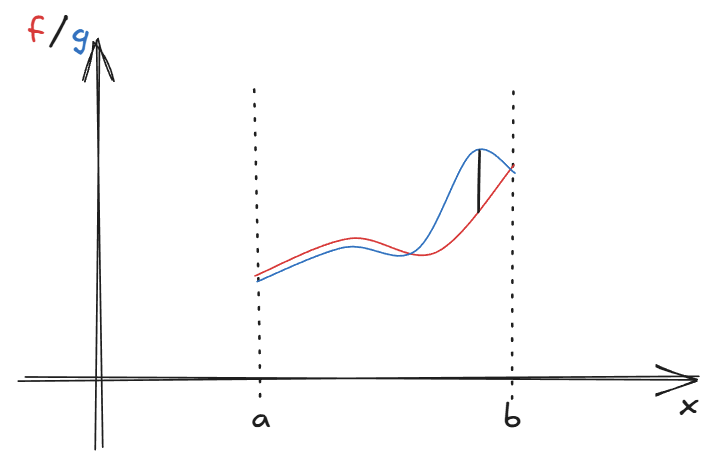
\includegraphics[width=0.6\linewidth]{chapters/part-2/figures/continuous-function-metric.png}
	\caption{A demonstrative example of a metric space defined on continuous functions.}
	\label{fig:continuous-function-metric}
\end{figure}

The proof of $(X,d)$ to be a metric space can be done fairly easily using the definition, and it is neglected here. 

The same idea applies to multivariable functions. It can also extend from continuous function $C^0$ to continuously differentiable functions $C^1$ (the function is differentiable and its differential is also continuous), in which case the distance function becomes
\begin{eqnarray}
	d(f,g) &=& \sup_{x\in[a,b]} |f(x)-g(x)| + \sup_{x\in[a,b]} |f\textprime(x)-g\textprime(x)| \nonumber
\end{eqnarray}
and to $n$-th order continuously differentiable function $C^n$, in which case the distance function becomes
\begin{eqnarray}
	d(f,g) &=& \sum_{i=0}^n \sup_{x\in[a,b]} |f^{(i)}(x)-g^{(i)}(x)| \label{eq:continuous-function-metric}
\end{eqnarray}

As for infinity-order continuously differentiable function $C^\infty$ which is also known as the \mync{smooth function}, \eqref{eq:continuous-function-metric} might be unbounded. Practically, we shall either limit the use of the metric to only bounded-distance smooth functions, or make a walk around with modified distance functions such as
\begin{eqnarray}
	d(f,g) &=& \sum_{i=0}^\infty 2^{-i}\dfrac{\sup_{x\in[a,b]} |f^{(i)}(x)-g^{(i)}(x)|}{1+\sup_{x\in[a,b]} |f^{(i)}(x)-g^{(i)}(x)|} \nonumber
\end{eqnarray}

Consider another metric space defined on continuous functions. Let $f,g \in C^0\left([a,b]\right)$ be two continuous functions on interval $[a,b]\subset \mathbb{R}$. Define the distance function $I_1:f \times g \to \mathbb{R}_{\geq 0}$ as follows.
\begin{eqnarray}
	I_1(f, g) &=& \int_{a}^{b} |f(x)-g(x)|dx \nonumber
\end{eqnarray}
It can be proved that the above forms a metric space.

The idea can be extended to the following series of distance functions, each corresponding with a metric space.
\begin{eqnarray}
	I_p(f, g) &=& \left(\int_{a}^{b} |f(x)-g(x)|^pdx\right)^{\frac{1}{p}} \label{eq:ipfg}
\end{eqnarray}
where $p\geq 1$. Under the scope of this notebook, only positive integer $p$ is considered.

Inspired by \eqref{eq:ipfg}, define the \mync{$L^p$ norm} of a continuous function as follows
\begin{eqnarray}
	\norm{f}_p &=& \left(\int_{a}^{b}|f(x)|^pdx\right)^{\frac{1}{p}} \nonumber
\end{eqnarray}
Continuous functions with bounded $L^p$ norm form an \mync{$L^p$ space}.






















